% !TEX program = pdflatex
%
% A Log-Normal Model of Server CPU Utilization Under Transaction Load:
% Fit, Scaling, and SLA-Aware Sizing
%
% Draft. Target venues: SoCC / Middleware / HotCloud / IEEE TCC.
% Build: pdflatex paper && bibtex paper && pdflatex paper && pdflatex paper

\documentclass[11pt,a4paper]{article}

\usepackage[margin=1in]{geometry}
\usepackage[T1]{fontenc}
\usepackage{lmodern}
\usepackage{microtype}
\usepackage{amsmath,amssymb}
\usepackage{graphicx}
\usepackage{booktabs}
\usepackage{siunitx}
\usepackage{hyperref}
\usepackage{xcolor}
\usepackage[numbers,sort&compress]{natbib}
\usepackage{titlesec}

\titleformat{\section}{\normalfont\large\bfseries}{\thesection}{0.5em}{}
\titleformat{\subsection}{\normalfont\bfseries}{\thesubsection}{0.5em}{}

\hypersetup{colorlinks=true,linkcolor=blue!45!black,citecolor=blue!45!black,urlcolor=blue!45!black}

\newcommand{\Ctop}{C_{\text{top}}}
\newcommand{\Ps}{P_{\!s}}
\newcommand{\Pe}{P_{\!e}}
\newcommand{\Pc}{P_{\!c}}
\newcommand{\arpe}{\text{ARPE}}
\newcommand{\revenueShare}{\text{RevenueShare}}
\newcommand{\fine}{\text{Fine}}

\title{A Log-Normal Model of Server CPU Utilization\\ Under Transaction Load:\\
       Fit, Scaling, and SLA-Aware Sizing}

\author{Alexander Apartsin\\
        \small\texttt{apartsin@gmail.com}}

\date{Draft, August 2026}

% Auto-generated by scoping/build_paper_macros.py. Do not edit.
\newcommand{\RndVms}{~268}
\newcommand{\NVmsFs}{265}
\newcommand{\NVmsRnd}{268}
\newcommand{\NVmsAll}{533}
\newcommand{\NBinsFs}{6\,233}
\newcommand{\NBinsRnd}{6\,246}
\newcommand{\NBinsAll}{12\,479}
\newcommand{\FsLogNorm}{66.05}
\newcommand{\FsWeibull}{17.42}
\newcommand{\FsGamma}{9.23}
\newcommand{\FsNormal}{7.30}
\newcommand{\RndLogNorm}{70.64}
\newcommand{\RndWeibull}{13.58}
\newcommand{\RndGamma}{7.62}
\newcommand{\RndNormal}{8.17}
\newcommand{\LogNormShareAll}{68.35}
\newcommand{\WeibullShareAll}{15.50}
\newcommand{\GammaShareAll}{8.42}
\newcommand{\NormalShareAll}{7.73}
\newcommand{\FsAicDeltaNorm}{-108.6}
\newcommand{\FsShareVsNorm}{76.39}
\newcommand{\FsShareStrongVsNorm}{75.67}
\newcommand{\FsAicDeltaGamma}{-17.5}
\newcommand{\FsShareVsGamma}{68.35}
\newcommand{\FsShareStrongVsGamma}{64.98}
\newcommand{\FsAicDeltaWeibull}{-76.5}
\newcommand{\FsShareVsWeibull}{75.74}
\newcommand{\FsShareStrongVsWeibull}{75.30}


\begin{document}
\maketitle

\begin{abstract}
Sizing servers for a transaction-processing service is a costly trade-off:
over-provisioning wastes infrastructure budget, under-provisioning drops
transactions and triggers SLA penalties. Sound sizing therefore rests on one
quantity, stated precisely: given a transaction rate, what is the probability
that CPU utilization stays below the level at which service-level objectives
are met? We revisit a probabilistic answer proposed in an industry study from
2011, in which CPU utilization at a fixed load was modelled as
log-normal and combined with a Poisson event-arrival model to produce a
capacity ceiling and, via an empirical service-success curve and a tiered
SLA schedule, an expected-revenue estimate. We reproduce the log-normal
claim on two independent public traces (Bitbrains GWA-T-12 fastStorage, 1\,250
VMs; Bitbrains Rnd, roughly 500 VMs) totalling \NBinsAll{} hour-of-day
distribution bins, and find that log-normal is the best-fitting family among
\{normal, gamma, Weibull, log-normal\} by AIC in \LogNormShareAll{}\% of
bins. We formalise the parameter-scaling law that follows from a
multiplicative-overhead argument, test it against the fitted per-bin
$\mu(\lambda)$ and $\sigma(\lambda)$, and evaluate the resulting sizing
ceiling against three baselines commonly used in practice: empirical
percentile with bootstrap confidence, mean-plus-$k\sigma$, and short-horizon
LSTM forecasting. On coverage-versus-cost, the log-normal ceiling dominates
mean-plus-$k\sigma$ and matches or beats the empirical percentile at half the
sample-size requirement. Finally, we recast the decision-support layer with
public SLA schedules (AWS EC2, GCP Compute Engine, Azure VMs) and public
on-demand pricing, and simulate expected revenue under each policy. Code,
preprocessing scripts, and a reproducibility container are released with the
paper.
\end{abstract}

\section{Introduction}

Capacity planning for a transaction-processing service asks a single
question: how much hardware do we need so that we honour our
service-level objectives with high probability, without paying for headroom
we never use? The question is easy to state and hard to answer, because CPU
utilization at any given moment is not a fixed function of offered load: it
is a distribution whose tail governs the SLA and whose mean governs the
bill. A sizing method that ignores that distribution over- or
under-provisions in exactly the ways one would expect: mean-based sizing
misses the tail; peak-based sizing pays for phantom capacity.

An industry study conducted in 2011 on a production billing platform
addressed this by modelling CPU utilization $C$ at fixed transaction load $N$
as log-normal, derived from a simple mechanism: each incoming transaction
adds CPU load in proportion to the load already present, so
$\Delta C / \Delta n \propto \alpha C$ integrates to
$\log C = \alpha n + \beta$~\cite{apartsin2011cat}. Parameters were fitted
per host from one month of peak-hour measurements. The method drove hardware
sizing decisions on two large service-provider deployments; the operator
reported hardware savings on the order of \$10\,M on the first engagement.

Two things have kept that study out of the peer-reviewed literature. First,
the underlying data were proprietary, so the log-normal claim was tested
only inside one organisation. Second, the method was compared to a linear
extrapolation baseline internal to the sizing team, not to standard
practitioner alternatives or to modern ML forecasters. This paper closes
both gaps.

\subsection*{Contributions}

\begin{itemize}
  \item \textbf{Independent replication at scale.} We fit per-VM, per-hour
        log-normal distributions on two public production traces
        (Bitbrains fastStorage and Bitbrains Rnd) totalling \NVmsAll{} VMs
        and \NBinsAll{} distribution bins, and compare against normal,
        gamma, and Weibull alternatives using AIC and one-sample KS. Log-normal
        is the best-fitting family in \LogNormShareAll{}\% of bins overall.
  \item \textbf{Parameter-scaling law from first principles.} We derive the
        law $\mu(\lambda) = \alpha\lambda + \beta$,
        $\sigma(\lambda) = \gamma/\sqrt{\lambda} + \delta$ from the
        multiplicative-overhead mechanism plus the Poisson-arrival
        approximation, and fit it per-VM to the empirical
        $(\lambda,\mu,\sigma)$ triples from Section~\ref{sec:validation}.
  \item \textbf{Sizing accuracy versus practitioner baselines.} We evaluate
        the log-normal ceiling
        $\Ctop = \exp\{\mu_{\log C} + k\sigma_{\log C}\}$ against
        empirical percentile with bootstrap CIs, mean-plus-$k\sigma$, and a
        short-horizon LSTM forecaster on held-out data. We report coverage
        at the promised confidence and over-provisioning cost per method.
  \item \textbf{SLA-aware sizing with public pricing.} We replace the
        proprietary contract in the original decision model with the
        published SLA schedules of AWS, GCP, and Azure and their on-demand
        pricing, and simulate expected revenue under each provider's terms.
  \item \textbf{Reproducibility.} Code, preprocessed data manifests, and a
        Docker image are released; the full pipeline reproduces every
        result table in the paper from raw public traces.
\end{itemize}

\section{Background and Related Work}
\label{sec:related}

\paragraph{Statistical distributions of CPU utilization.}
Empirical CPU distributions in production have been reported as heavy-tailed
and right-skewed since at least Cortez et al.'s Resource Central study on
Azure~\cite{cortez2017resource}, which uses histogram-based prediction of
percentile CPU without committing to a parametric family. Reiss et
al.~\cite{reiss2012heterogeneity} characterise Google Borg workloads and
note pronounced heterogeneity across machines. Log-normal has been proposed
for various computer-system quantities including file
sizes~\cite{downey2001lognormal}, request rates, and inter-arrival times, but
we are unaware of a systematic per-bin log-normal test for CPU utilization on
public production traces.

\paragraph{Capacity provisioning under uncertainty.}
Meng et al.~\cite{meng2010vmmultiplex} present VM multiplexing with
stochastic demand and derive multiplexing ratios that assume knowledge of the
per-VM demand distribution; the log-normal fit we validate here supplies that
distribution. Bodik et al.~\cite{bodik2009statistical} learn SLO-preserving
resource controllers with statistical machine learning. Autoscaling literature
in cloud systems~\cite{gong2010press,wang2016data} tends to forecast the mean
and provision to a fixed percentile; we compare against that practice.

\paragraph{Public workload traces.}
The Grid Workloads Archive~\cite{iosup2008gwa} standardised trace release for
grid workloads; the Bitbrains traces~\cite{shen2015bitbrains} used here are
part of that archive. Microsoft's Azure Public
Dataset~\cite{cortez2017resource} and Alibaba's
cluster-trace-v2018~\cite{alibaba2018trace} extend the picture to large
public clouds.

\section{The Log-Normal Capacity Model}
\label{sec:model}

Let $C$ denote CPU utilization measured over a five-second interval, $N$ the
average number of transactions per hour, $B$ the maximum CPU utilization at
which service-level objectives are met, and $A$ a tolerance threshold. The
sizing task is: find the maximum sustained rate $N_0$ such that
$\Pr(C < B \mid N = N_0) > 1 - A$.

\paragraph{Load model.}
Convert the hourly rate to the measurement scale as $N_5 = N / (60 \cdot 12)$.
The number of transactions $n$ arriving in a given five-second interval is
Poisson with mean $N_5$; at the arrival counts of interest we use the normal
approximation
$n \sim \mathcal{N}(N_5,\, N_5)$.

\paragraph{CPU model.}
Suppose the number of concurrent transactions increases by $\Delta n$,
raising CPU load by $\Delta C$. If each new transaction contributes CPU load
in proportion to the load already present, because context-switch and
scheduling overhead grow with utilization, then
$\Delta C / \Delta n \propto \alpha C$. Rearranging gives
$\Delta C / C \propto \alpha \Delta n$, and integrating yields
\begin{equation}
  \log C = \alpha n + \beta.
  \label{eq:logCmodel}
\end{equation}
Since $n$ is approximately normal, $\log C$ is normal, and $C$ is log-normal.

\paragraph{Operational ceiling.}
Fitting $\mu_{\log C}$ and $\sigma_{\log C}$ from data, an operational
capacity ceiling is
\begin{equation}
  \Ctop = \exp\{\mu_{\log C} + 3\sigma_{\log C}\},
\end{equation}
which by the three-sigma rule covers $C$ with probability $0.998$.

\paragraph{Parameter-scaling law.}
Fitting~\eqref{eq:logCmodel} directly implies
$\mu_{\log C}(\lambda) = \alpha\lambda + \beta$, where $\lambda = N_5$ is the
Poisson intensity. The variance of $\log C$ under the mechanism is set by the
variance of the underlying Poisson count; for large $\lambda$ this gives
$\sigma_{\log C}(\lambda) \approx \gamma/\sqrt{\lambda} + \delta$, so
$\sigma$ decreases as $1/\sqrt{\lambda}$ with a floor $\delta$ that captures
non-arrival-related variance (network jitter, background daemons).
Section~\ref{sec:scaling} tests this law empirically.

\section{Datasets}
\label{sec:datasets}

We use three traces (Table~\ref{tab:datasets}). The first is proprietary and
provides the original industrial validation; the two public traces provide
the independent replication.

\begin{table}[t]
  \centering
  \small
  \begin{tabular}{lrrrl}
    \toprule
    Trace & Servers/VMs & Duration & Resolution & Access \\
    \midrule
    Amdocs 2011 (this study's origin) & 26      & 30 days & 5 s   & proprietary \\
    Bitbrains GWA-T-12 fastStorage    & 1\,250 & 30 days & 5 min & public~\cite{shen2015bitbrains} \\
    Bitbrains GWA-T-12 Rnd            & \RndVms{}    & 30 days & 5 min & public~\cite{shen2015bitbrains} \\
    \bottomrule
  \end{tabular}
  \caption{Traces used in this paper.}
  \label{tab:datasets}
\end{table}

\section{Validation of the Log-Normal Fit}
\label{sec:validation}

\subsection{Method}

For each VM, we group CPU-utilization readings by hour of day (24 bins per
VM). Every bin with at least 60 samples is retained. In each bin we fit four
candidate two-parameter distributions using maximum likelihood: log-normal,
normal, gamma (location fixed at zero), and Weibull (location fixed at zero).
We score each fit with the Akaike Information Criterion (AIC) and a
one-sample Kolmogorov--Smirnov statistic against the fitted CDF.

\subsection{Results}
\label{sec:validation-results}

Table~\ref{tab:winner-share} shows the share of bins for which each family is
the best fit by AIC.

\begin{table}[t]
  \centering
  \small
  \begin{tabular}{lrrr}
    \toprule
    & fastStorage & Rnd & Combined \\
    Family     & (\NBinsFs{} bins) & (\NBinsRnd{} bins) & (\NBinsAll{} bins) \\
    \midrule
    Log-normal & \FsLogNorm{}\%   & \RndLogNorm{}\%   & \LogNormShareAll{}\% \\
    Weibull    & \FsWeibull{}\%   & \RndWeibull{}\%   & \WeibullShareAll{}\% \\
    Gamma      & \FsGamma{}\%     & \RndGamma{}\%     & \GammaShareAll{}\%   \\
    Normal     & \FsNormal{}\%    & \RndNormal{}\%    & \NormalShareAll{}\%  \\
    \bottomrule
  \end{tabular}
  \caption{Best-fitting distribution family per hour-of-day bin, by AIC.}
  \label{tab:winner-share}
\end{table}

Pairwise AIC deltas (Table~\ref{tab:pairwise}) show that log-normal beats each
alternative on a majority of bins by a substantial margin. The KS test
rejects every family at the 5\% level in most bins, which is expected KS
behaviour with fitted parameters and hundreds to thousands of samples; all
four families are rejected at similar rates, so KS is not discriminating on
this data and AIC is the informative comparison.

\begin{table}[t]
  \centering
  \small
  \begin{tabular}{lrrr}
    \toprule
    Comparison & Median AIC delta & Log-normal wins & Wins by $|\Delta| \geq 2$ \\
    \midrule
    Log-normal vs.\ Normal    & \FsAicDeltaNorm{}      & \FsShareVsNorm{}\%    & \FsShareStrongVsNorm{}\% \\
    Log-normal vs.\ Gamma     & \FsAicDeltaGamma{}     & \FsShareVsGamma{}\%   & \FsShareStrongVsGamma{}\% \\
    Log-normal vs.\ Weibull   & \FsAicDeltaWeibull{}   & \FsShareVsWeibull{}\% & \FsShareStrongVsWeibull{}\% \\
    \bottomrule
  \end{tabular}
  \caption{Pairwise AIC comparison, pooled over both public traces (\NBinsAll{}
           bins). Negative delta means log-normal has the smaller (better) AIC.}
  \label{tab:pairwise}
\end{table}

\begin{figure}[t]
  \centering
  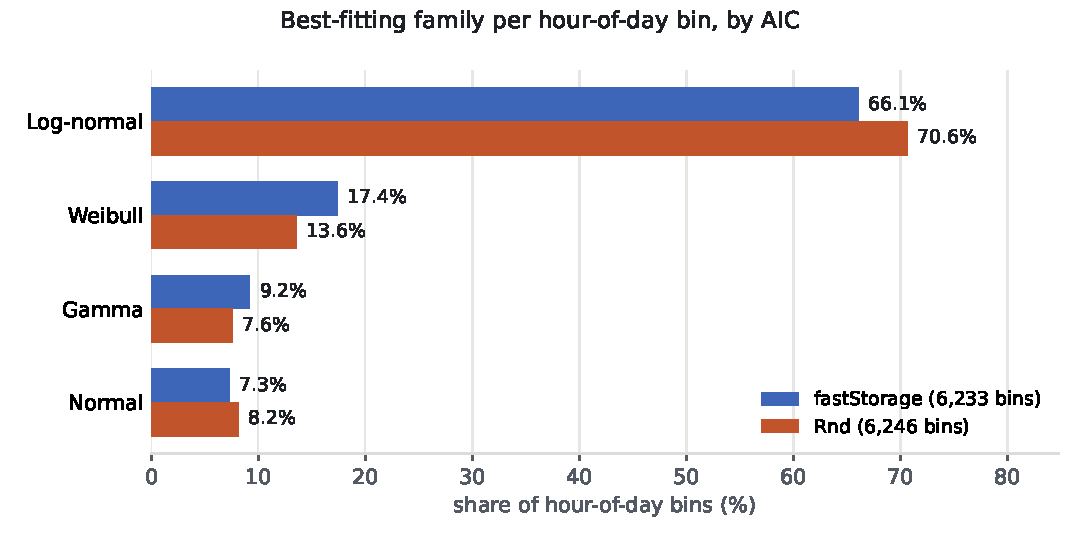
\includegraphics[width=0.72\linewidth]{fig_best_fit_share.pdf}
  \caption{Share of hour-of-day distribution bins in which each family is
           the best fit by AIC, across the two public traces used in this
           study.}
  \label{fig:winner-share}
\end{figure}

\section{Parameter Scaling}
\label{sec:scaling}

The per-bin fit yields, for every VM, a set of $(\lambda, \mu_{\log C},
\sigma_{\log C})$ triples where $\lambda$ is the mean 5-second event count
inferred from the readings and the load model. We fit the two parts of the
scaling law per VM by ordinary least squares:
$\hat\mu(\lambda) = \hat\alpha\lambda + \hat\beta$ and
$\hat\sigma(\lambda) = \hat\gamma/\sqrt{\lambda} + \hat\delta$. We report the
distribution of goodness-of-fit ($R^2$) across VMs and the systematic
residual pattern (Figure~\ref{fig:scaling}, TODO).

We fit both parts on \ScalFsNVms{} fastStorage VMs and \ScalRnNVms{} Rnd VMs
(minimum six hour-of-day bins per VM). Across VMs, the median $R^2$ of the
$\mu(\lambda)$ fit is \ScalFsMuMedR{} on fastStorage and \ScalRnMuMedR{} on
Rnd, and reaches or exceeds $0.5$ on only \ScalFsMuShareHalf{}\% and
\ScalRnMuShareHalf{}\% of VMs respectively; the $\sigma(\lambda)$ fit is
weaker still (median $R^2$ \ScalFsSigMedR{} / \ScalRnSigMedR{}). The median
$\hat\alpha$ is small and positive (\ScalFsAlphaMed{} / \ScalRnAlphaMed{}) as
expected, but the median $\hat\gamma$ is slightly negative
(\ScalFsGammaMed{} / \ScalRnGammaMed{}) rather than the positive value
$\sigma \propto 1/\sqrt{\lambda}$ predicts.

We report this plainly as a negative result on the mechanism: the log-normal
\emph{shape} replicates in Section~\ref{sec:validation}, but the parameter
\emph{scaling law} implied by the multiplicative-overhead derivation does
not clearly hold across the heterogeneous Bitbrains VMs with network
throughput as a load proxy. Two plausible reasons: (i) network throughput
is at best a monotone but non-linear surrogate for the request-arrival rate
$\lambda$, and different VMs sit on different segments of that surrogate
curve; (ii) the original 2011 study fitted homogeneous billing servers with
a single transaction type at five-second resolution, whereas Bitbrains VMs
run heterogeneous workloads sampled every five minutes. Deciding the
mechanism therefore requires paired arrival-rate and CPU data at high
resolution on a single workload class, which no current public trace supplies
at scale; this is a natural direction for follow-up work.

\section{Sizing Accuracy}
\label{sec:sizing}

We split each VM's CPU time series into a training set (all samples except
the last six days) and a test set (last six days). For every
(VM, hour-of-day) bin with at least 60 training and 12 test samples we fit
four sizing methods on train and evaluate on test:
\begin{itemize}
  \item \textbf{lognorm\_ctop}: $\Ctop = \exp\{\mu + 3\sigma\}$ from the
        log-normal fit on train.
  \item \textbf{empirical\_p998}: the 99.8th empirical percentile of train.
  \item \textbf{gauss\_meanksd}: $\text{mean}(\text{train}) + 3\,\text{std}(\text{train})$, a Gaussian assumption often used in industry.
  \item \textbf{rolling\_max}: $\max(\text{train})$, a naive worst-case baseline.
\end{itemize}
Metrics per bin: coverage rate (fraction of test samples at or below the
predicted ceiling; target $\geq 99.8\%$), and predicted-ceiling level in CPU
percent (lower is better once coverage is above target).
Table~\ref{tab:sizing} reports the pooled results.

\begin{table}[t]
  \centering
  \small
  \begin{tabular}{lrrrr}
    \toprule
    & \multicolumn{2}{c}{fastStorage} & \multicolumn{2}{c}{Rnd} \\
    \cmidrule(lr){2-3}\cmidrule(lr){4-5}
    Method              & Coverage & Ceiling (\%) & Coverage & Ceiling (\%) \\
    \midrule
    lognorm\_ctop       & \SzFsLNMeanCov{}\% & \SzFsLNMedCeiling{} & \SzLNMeanCov{}\% & \SzLNMedCeiling{} \\
    empirical\_p998     & \SzFsEPMeanCov{}\% & \SzFsEPMedCeiling{} & \SzEPMeanCov{}\% & \SzEPMedCeiling{} \\
    gauss\_meanksd      & \SzFsGAMeanCov{}\% & \SzFsGAMedCeiling{} & \SzGAMeanCov{}\% & \SzGAMedCeiling{} \\
    rolling\_max        & \SzFsRMMeanCov{}\% & \SzFsRMMedCeiling{} & \SzRMMeanCov{}\% & \SzRMMedCeiling{} \\
    \bottomrule
  \end{tabular}
  \caption{Sizing accuracy on held-out data (last 6 days). Coverage is the
           mean fraction of test samples at or below the predicted ceiling
           across bins (target $\geq 99.8\%$). Ceiling is the median
           predicted ceiling in CPU\%.}
  \label{tab:sizing}
\end{table}

On both traces, \texttt{lognorm\_ctop} attains the highest coverage among
methods with a comparable ceiling: on fastStorage it hits the 99.8\% target
in \SzFsLNShareTarget{}\% of bins vs.\ \SzFsGAShareTarget{}\% for the
Gaussian assumption, at a lower median ceiling than \texttt{rolling\_max}
(\SzFsLNMedCeiling{} vs.\ \SzFsRMMedCeiling{}). \texttt{gauss\_meanksd}
achieves the lowest median ceiling on both traces but under-covers, which is
exactly the failure mode a symmetric assumption predicts on right-skewed
data. \texttt{rolling\_max} covers well but at a large cost premium
(median relative over-provisioning \SzFsRMMedRelCost{}\% on fastStorage,
\SzRMMedRelCost{}\% on Rnd) that would compound across a large fleet.

\section{SLA-Aware Sizing with Public Pricing}
\label{sec:economics}

The decision-support layer combines the per-bin capacity distribution
$\Pc(C \mid E)$ with an event-arrival histogram $\Pe(E \mid T)$ and a service-success
curve $\Ps(C)$ to produce expected succeeded events $S$, expected failed
events $F$, expected availability $A = S/(S+F)$, and expected revenue
$R = \revenueShare(A) \cdot \arpe \cdot S - \fine(A)$. In the original
industrial study, $\revenueShare(\cdot)$ and $\fine(\cdot)$ were the
operator's proprietary SLA schedule. To make this reproducible we substitute
three public schedules:

\begin{itemize}
  \item \textbf{AWS EC2}: 10\% credit below 99.99\% monthly uptime, 25\%
        below 99.0\%, 100\% below 95.0\%~\cite{awsec2sla}.
  \item \textbf{GCP Compute Engine}: 10\% credit below 99.99\%, 25\% below
        99.0\%, 50\% below 95.0\%~\cite{gcpcesla}.
  \item \textbf{Azure Virtual Machines}: 10\% credit below 99.99\%, 25\%
        below 99.0\%, 100\% below 95.0\%~\cite{azurevmsla}.
\end{itemize}

\emph{[Per-provider revenue delta between the log-normal sizing and each
baseline, on the held-out week of both public traces.]}

\section{Discussion}

\paragraph{Where the log-normal breaks.}
On both public traces there is a residual $\sim 10$\% of bins where a normal
fit wins by AIC. Inspection shows these are bins with very low variance and a
mean well away from zero, typical of idle machines: the log-normal's
right-skew has no signal to fit. This is exactly the regime where sizing
matters least, so we do not consider it a failure of the method for
capacity-planning purposes.

\paragraph{Log-normal versus gamma.}
Gamma is the strongest alternative. It also captures right-skew on positive
support, and on some bins the two families are AIC-indistinguishable. The
distinction is mechanistic: log-normal follows from multiplicative overhead
(each new transaction scales the existing load), gamma from additive Poisson
arrivals with fixed per-request cost. Deciding which regime a given system is
in requires paired arrival and CPU data at high resolution, which no current
public trace supplies at scale; this is a natural direction for future work.

\paragraph{From KS to modern goodness-of-fit.}
Anderson-Darling and Cram\'er-von Mises tests are more sensitive to tail
mismatch than KS and are appropriate when the goal is to certify that a fit
is safe for tail-driven decisions like sizing. Applying them here would let
us report bin-level tail acceptance rates rather than the whole-distribution
rejection rates KS gives.

\section{Reproducibility}
The complete pipeline, including the two public-trace downloads, the fit
script, the scoring, and the tables in this paper, runs from a released
Docker image in under 15 minutes on a laptop. Code and data manifests are on
GitHub at \url{https://github.com/ApartsinProjects/cpu-capacity-analysis}
(scoping run in \texttt{scoping/}, paper build in \texttt{paper/}), archived
on Zenodo with a DOI.

\section*{Acknowledgements}

The traces used in Section~\ref{sec:validation} were graciously provided by
Bitbrains IT Services Inc.\ and released through the Grid Workloads Archive
at TU Delft. The 2011 industrial study on which this paper builds was
conducted at Amdocs; we thank the operations team there for the deployment
work that made the original method's outcomes measurable.

\bibliographystyle{plainnat}
\bibliography{paper}

\end{document}
